\chapter{Measuring the Cosmic Microwave Background}

%todo include continuous reading of angle and power data, maybe using video?

%todo build up to this lab using blackbody lab with light bulbs? Maybe this device and different temperatures of light bulbs and spectrometers?

\section*{Introduction}

In this experiment we will perform a measurement first carried out in the mid 1960s by Arno Penzias and Robert Wilson, for which they shared the 1978 Physics Nobel Prize for the discovery of the Cosmic Microwave Background Radiation.\footnote{A note on the Penzias and Wilson Nobel-prize winning measurement can be found at: \url{http://www.bell-labs.com/project/feature/archives/cosmology/}.}  We will measure the temperature of the Cosmic Microwave Background Radiation by comparing the  power of this emission directly with the emission from thermal sources in the lab. 

\begin{figure}[htbp]
	\begin{center}
		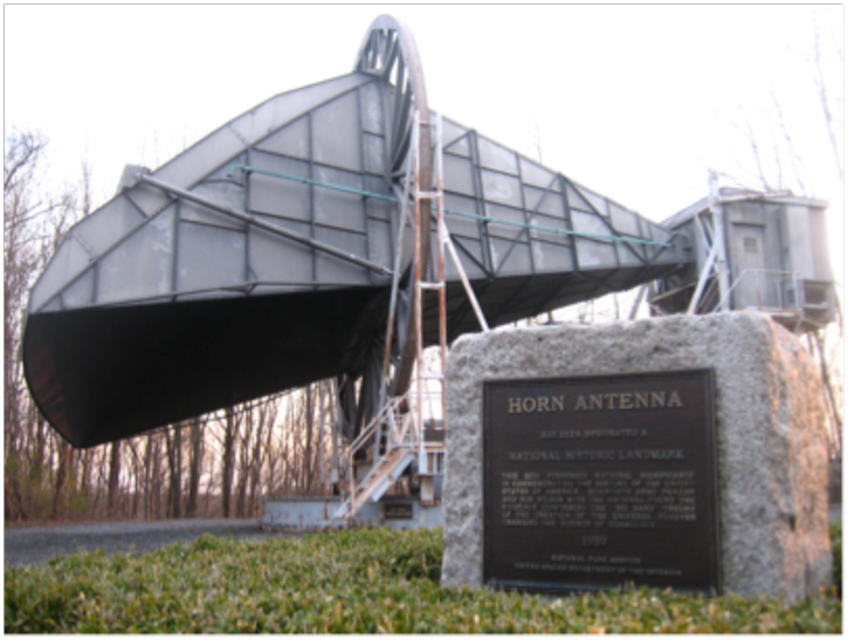
\includegraphics[width=.45\textwidth]{cmb/CMB-horn-antenna.pdf}
		\caption{A photo of the horn antenna with which Arno Penzias and Robert Wilson discovered the Cosmic Microwave Background radiation. This lab uses a smaller horn working at a much higher frequency (shorter wavelength), so that the ``beam patterns" are similar (recall the Small Radio Telescope lab and beam measurements to see why). }
		\label{fig:PW-horn}
	\end{center}
\end{figure}

\section{Measuring Temperatures with Thermal Radiation}

We use the basic fact that at sufficiently long wavelengths, the power emitted by a perfect thermal emitter is proportional to the temperature of the emitter:
\begin{equation}
P = \alpha T
\label{one}
\end{equation}
where $P$ is the power emitted, $\alpha$ is a constant that depends on area, wavelength, and other factors, and $T$ is the physical temperature of the emitter in Kelvin. 

To measure the power we use an instrument that can measure the incoming radiation power and it has input optics arranged so that it ``views'' a small range of angles in front of the instrument. This is the basis of a radiometer. You can imagine this as a reverse flashlight. In the case of the flashlight, the filament of the light bulb is hot and emits through an arrangement of mirrors to form a narrow beam. For the radiometer, the ``heat radiation'' from a narrow range of angles funnels into the instrument and the power is detected and the amount of power read out on a meter.

In practice, the receiver used to measure radiation is not perfect and generates some `noise' power of its own. So even if we pointed the receiver at an object with $T=0$, it would still measure some power. This extra power is denoted in terms of the temperature, $T_\textrm{rx}$, you would measure if you looked at a zero temperature emitter and did not correct for this fact:
\begin{equation}
P = \alpha (T + T_\textrm{rx}).
\label{two}
\end{equation}

To compute temperature of an emitter, $T$, from the power, $P$, measured by receiver, we need to know $\alpha$ and $T_\textrm{rx}$. 
It would be hard to calculate the factor $\alpha$ from first principles, especially because in order to be useful the calculation must include all of the details of the measuring equipment.  However, it is straightforward to obtain an accurate measurement of  $\alpha$ experimentally by measuring the power for different temperatures.

We will determine the factor $\alpha$ by placing first an emitter of one known temperature in front of the radiometer, noting the power reading on the meter, then placing a different emitter with a different known temperature in front of the radiometer and noting the new power level. According to equations~\ref{one} and \ref{two}, these two measurements can be used to calculate $\alpha$:
\begin{equation}
\alpha = {P_1 - P_2 \over T_1 - T_2}
\label{three}
\end{equation}

Once $\alpha$ is calculated, we can solve for $T_\textrm{rx}$ from measurement of one of the known temperature emitters:
\begin{equation}
T_\textrm{rx} = {P_1 \over \alpha} -T_1
\label{four}
\end{equation}
With $\alpha$ and $T_\textrm{rx}$ measured, we can ``point'' the radiometer anywhere and remotely measure the temperature of any emitter corresponding to the received power $P$ by solving eq.~\ref{two}  for $T$,

\begin{equation}
T={P\over \alpha} - T_\textrm{rx}
\label{five}
\end{equation}

Note that when you will be measuring the temperature of the ``hot'' load you will need to convert the temperature in degrees Celsius or Fahrenheit it reports into Kelvins.

\section{The receiver and experimental set up}

Figure~\ref{fig:CMBLab-photo} shows the experimental set up you will be using in this lab. The 30 GHz receiver is enclosed in a cryostat enclosure that keeps it very cold to reduce its noise. It is mounted on a cart in a contraption that allows to change its pointing for different elevations. Radiation measured by the receiver enters through receiver window at the top of the enclosure. The power measured by the receiver is displayed in digital form on the power readout screen. Pointing of the receiver can be changed using the elevation control lever and current elevation can be read on the electronic angle meter mounted on the enclose (this meter should be calibrated at the zero angle at the beginning of the lab with the help of your TA).

Figure~\ref{fig:schematic} shows details of the receiver when it is taken out of the cryostat enclosure.

\begin{figure}[ht]
	\begin{center}
		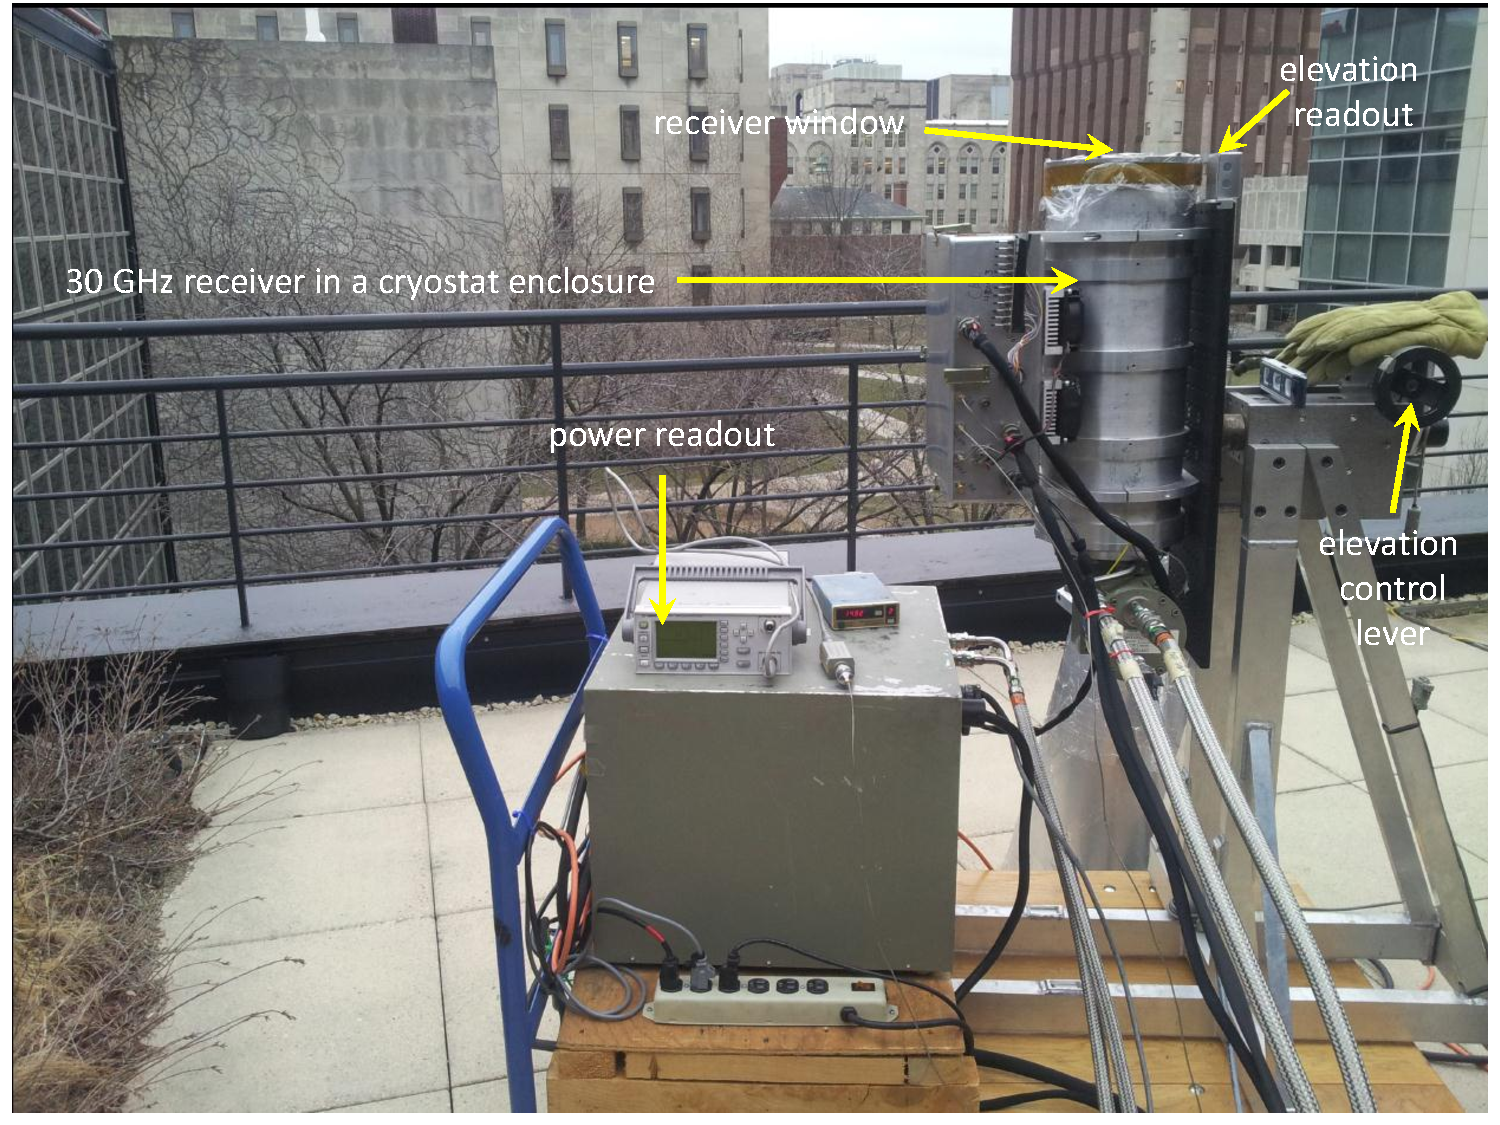
\includegraphics[trim=0pt 0pt 0pt 0pt,width=0.9\textwidth]{cmb/receiver_setup_new.pdf}
		\caption{Photo of the 30 GHz receiver enclosed in a cryostat enclosure mounted on the cart. This set up on a patio of KPTC 312 will be used in this lab for measurements of temperature of the sky.}
		\label{fig:CMBLab-photo}
	\end{center}
\end{figure}

\begin{figure}[htb]
	\begin{center}
		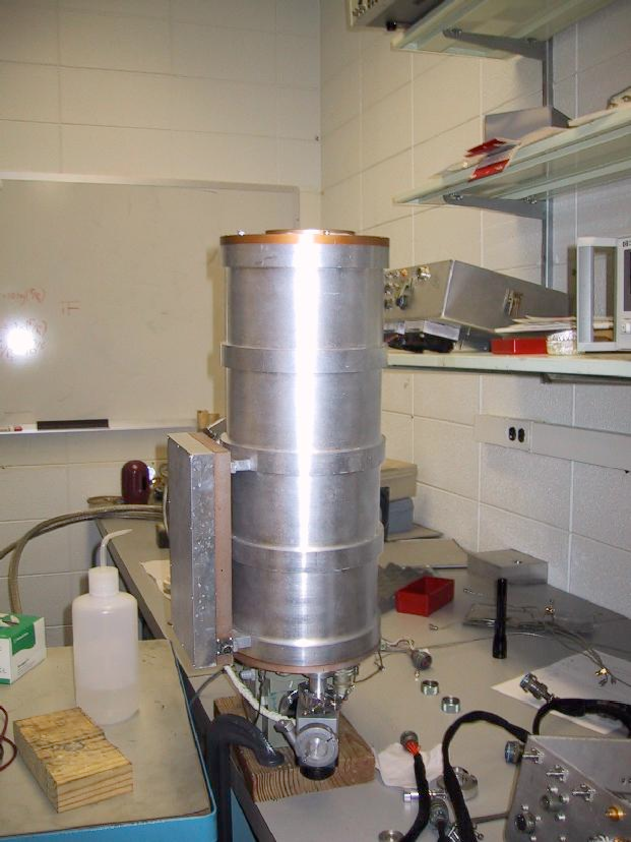
\includegraphics[trim=0pt 0pt 0pt 0pt,width=0.4\textwidth]{cmb/SZ-Cryostat-Closed.pdf}
		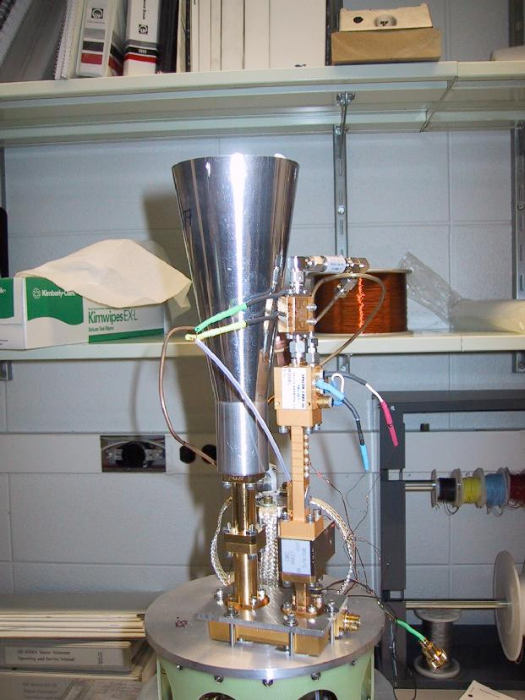
\includegraphics[trim=0pt 0pt 0pt 0pt,width=0.4\textwidth]{cmb/SZ-Cryostat-Open.pdf}
		\caption{\textit{Left:} The CMB lab 30 GHz receiver closed in the lab. \textit{Right:} A photo of the inside of the cryostat showing the  horn and electronics of the receiver.  The outer shell of the cryostat provides the vacuum seal for the interior components that are cooled to roughly 15 K (-258 C) inside of thermal radiation shields (not shown) to lower the noise generated by the electronics, and even the noise due to the radiation from the horn. The electronics amplify the signal by roughly a factor of 10,000.  By cooling and using a specially designed amplifier for this research, the receiver only adds a small amount of noise, roughly equivalent to that which would result by placing 10 K at the input of an idealized noiseless receiver (if only such things existed!). This receiver  was built here at the university and is also used to at the CARMA radio astronomy observatory, see \url{http://www.mmarray.org/}, for which The University of Chicago is a partner. It is one of a handful of the most sensitive 30 GHz receivers in the world.}
		\label{fig:schematic}
	\end{center}
\end{figure}

\section{Measuring the Temperature of Items in the Lab}

We will first measure the temperature of several items using the radiometer. 

Some things you could measure: 
\begin{enumerate}
	\item The wall or ceiling
	\item The sky through the door of the lab
	\item Your cupped hands above the receiver or your face
\end{enumerate}

For each item, you should make three or more measurements quickly in succession of the cold load, the hot load, and the source for which you want to measure temperature. The hot load is a piece of material that is a good emitter and the temperature is near room temperature and is measured with a a digital thermometer located at the top of the load (see left panel of Fig.~\ref{fig:details}). The cold load is a similar material that is first immersed completely in liquid Nitrogen (which has temperature $T_\textrm{cold}=77.4$~K),\footnote{It is important that the entire cone is immersed in the liquid Nitrogen or else the effective temperature of the load will be poorly determined and this will lead to incorrect measurement of the source temperature.} as shown in the middle panel of Fig.~\ref{fig:details}. When you are ready to make a measurement with the cold load, take it out of the dewar, let the liquid Nitrogen drip for $\sim$5 seconds and place it in front of the receiver window. Be careful to fully cover the window, but do not rest the cold load on the cryostat. Then comes the source of unknown temperature. For each of these objects you will need to read the power reading on the power meter attached to the receiver (see Fig.~1).

Find the unknown temperature using equation~\ref{two} to find $\alpha$, equation~\ref{four} to find $T_\textrm{rx}$, with $T_1$ and $P_1$ being the temperature and power for the hot load, $T_2$ and $P_2$ being the temperature and power for the cold load. Then using equation~\ref{five}, find the unknown temperature using the power measured while the unknown was in front of the receiver.

\begin{figure}[ht!]
	\begin{center}
		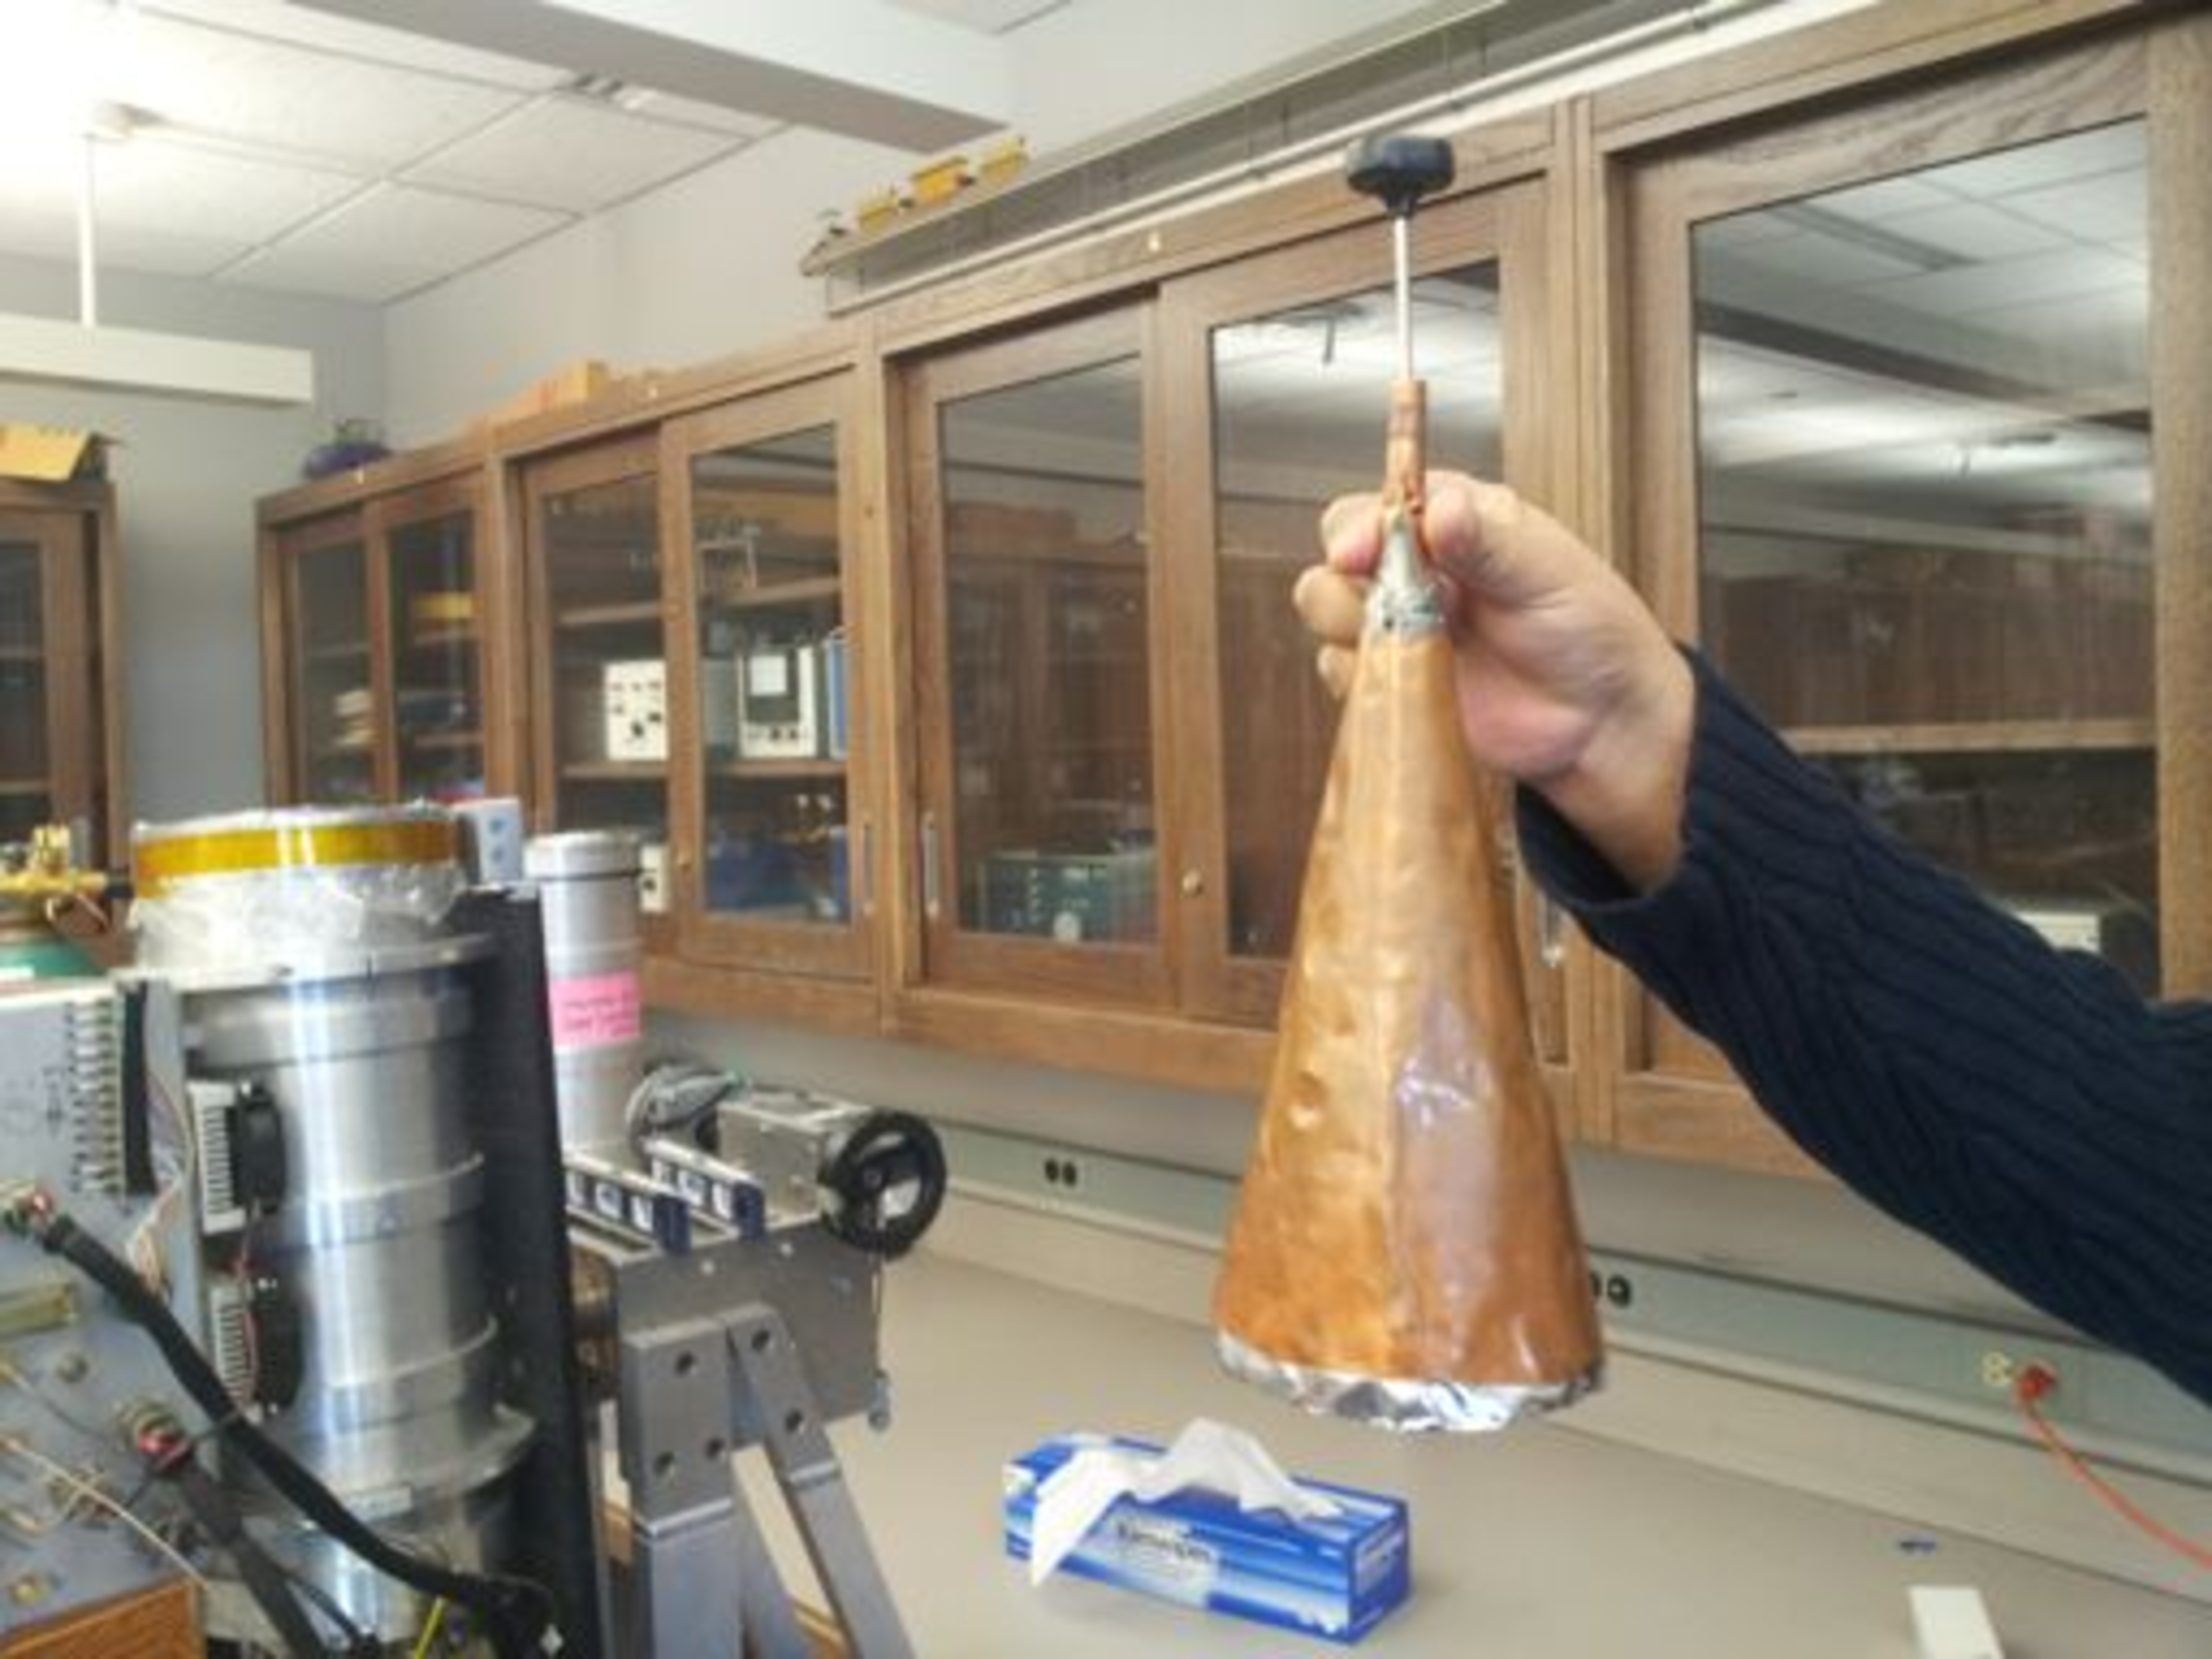
\includegraphics[trim=0pt 0pt 0pt 0pt,width=0.32\textwidth]{cmb/hot_load-small.pdf}
		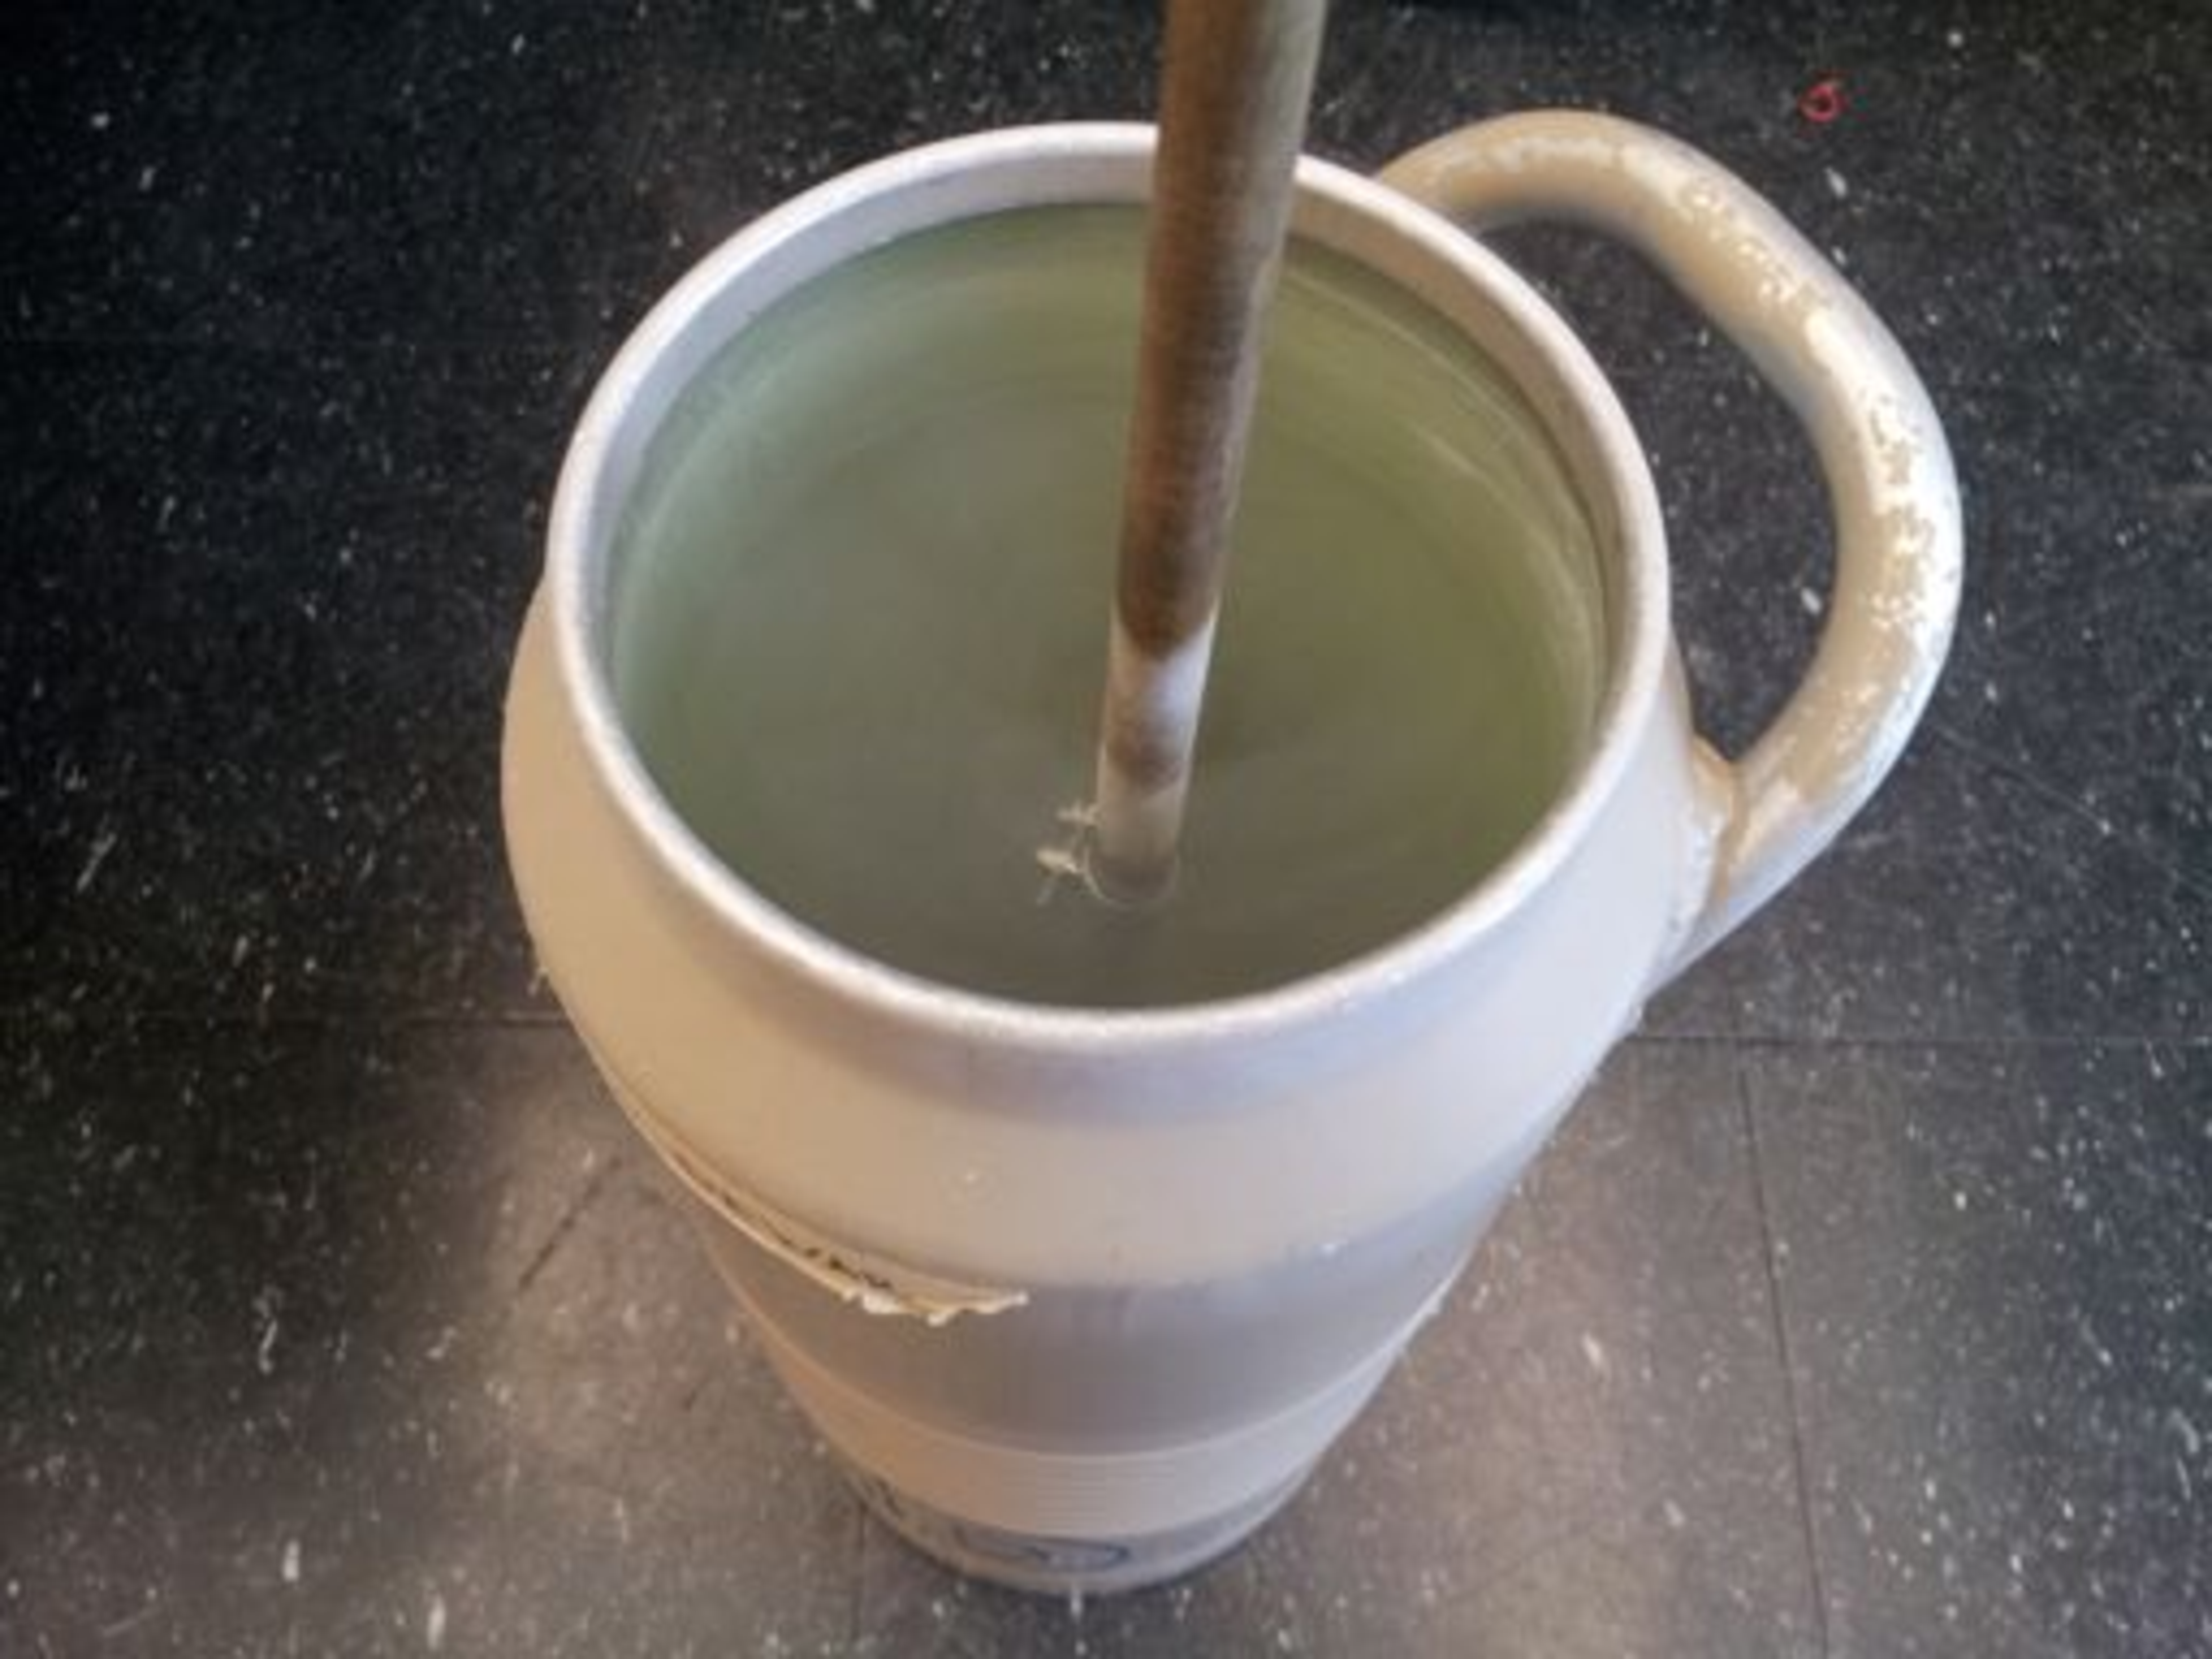
\includegraphics[trim=0pt 0pt 0pt 0pt,width=0.32\textwidth]{cmb/cold_load-small.pdf}
		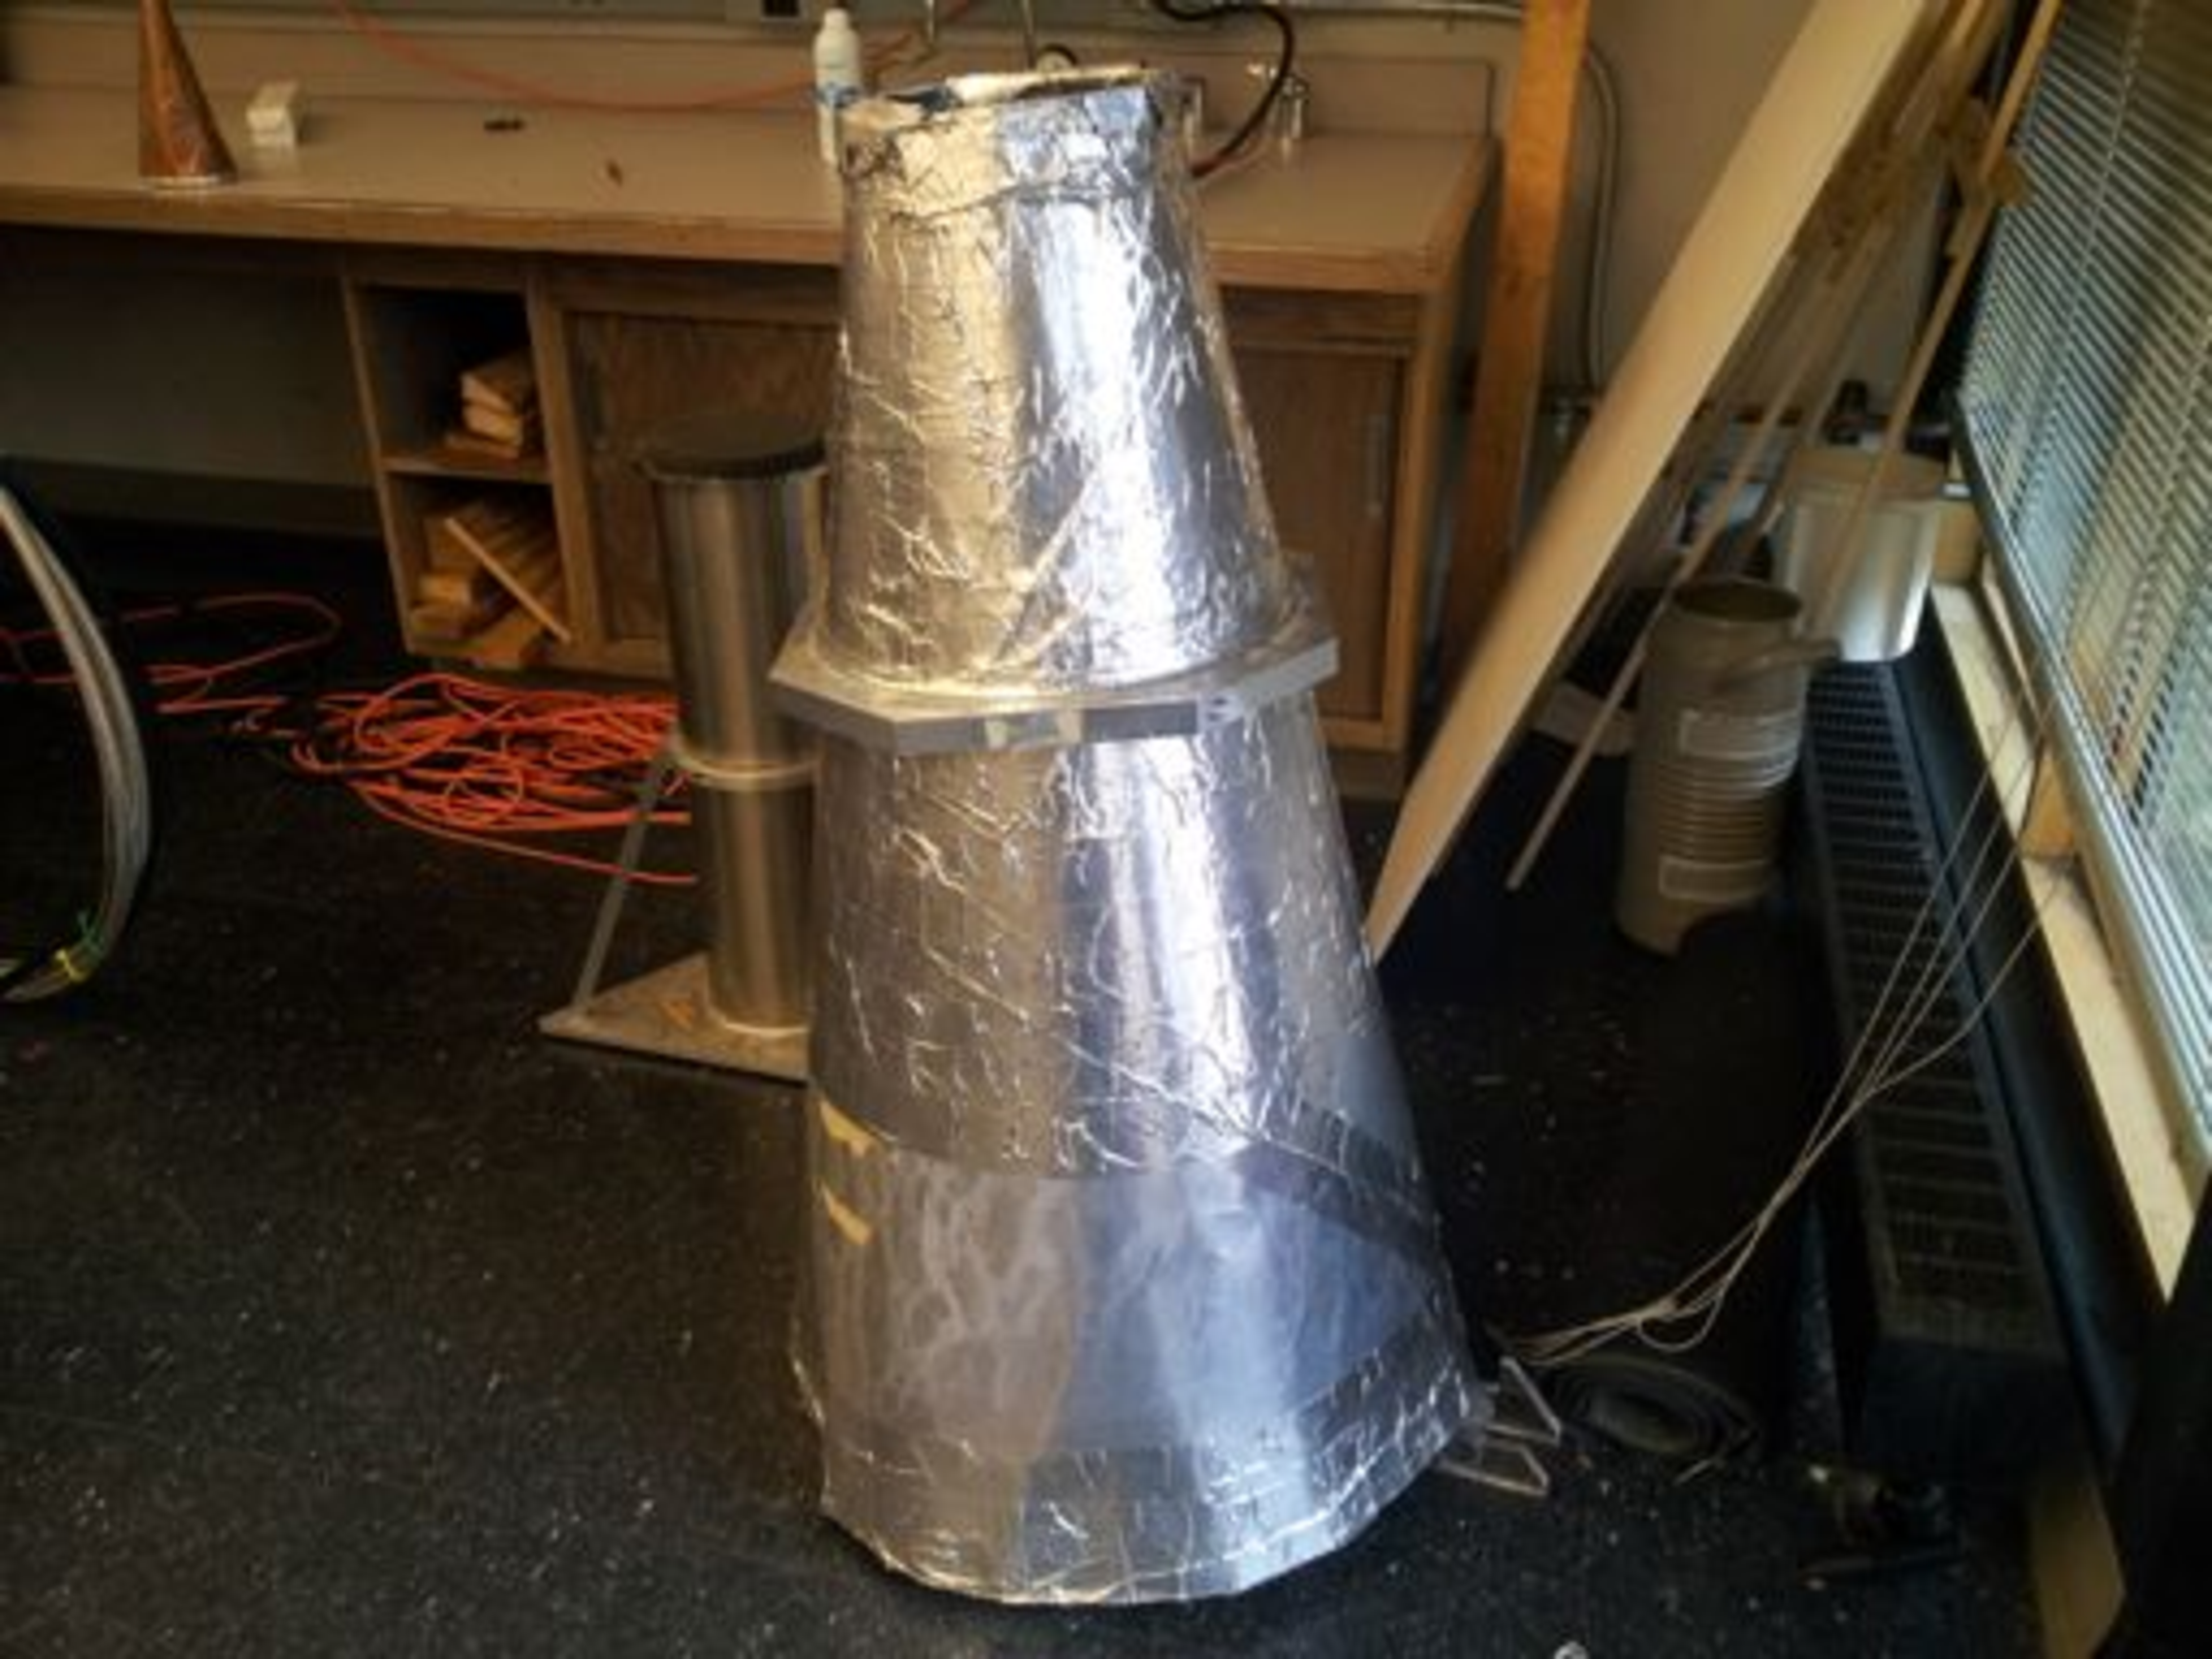
\includegraphics[trim=0pt 0pt 0pt 0pt,width=0.32\textwidth]{cmb/ground_shield-small.pdf}
		\caption{\textit{Left:} The ``hot'' load with digital thermometer at the top. \textit{Center:} ``cold'' load submerged in a dewar with liquid Nitrogen. Make sure that the cooper part of the load is fully submerged with the liquid surface at a wooden part of the load. \textit{Right:} ground shield which will be used to minimize radiation from nearby buildings  and the ground when measuring radiation from the sky. } 
		\label{fig:details}
	\end{center}
\end{figure}

\section{Measuring the Temperature of the CMB}

Measuring the temperature of the CMB is conceptually the same as  measuring the temperature of the items in the lab. We will compare the power we get from the sky to the hot and cold loads.

Because the CMB temperature is very low (just a few degrees K) we have to take a more careful account of a few things than we did for the previous section. First, we will have to get $T_\textrm{rx}$ pretty accurately because the CMB temperature, $T_\textrm{CMB}$ is less than $T_\textrm{rx}$. Second, there are hot sources (compared to the CMB) all around the experiment. You can imagine that even a small bit of one of these hot sources in part of the beam would change the oncoming power a lot and cause a big change in what we infer for the CMB temperature. 

We will also have to worry about two other sources.
One is the hot ground and buildings around us. We will guess about these sources by placing a ground shield on the receiver, which keeps the ground emission out of the input (see right panel of Fig.~\ref{fig:details} to see how the ground shield looks like). We will check how much difference this makes and subtract that source if it seems to be an important factor.

The second, and more difficult extraneous source to remove is emission from our own atmosphere. While the atmosphere is \textit{almost} transparent (and therefore almost non-emissive), it is not perfect. What's more, the main emitter is water-vapor which varies a lot. There is not much water vapor on those clear, crisp days when the sky is deep blue. On the other hand, when it's wet and cloudy, there is a lot of water vapor, and consequently, if we point our radiometer up at the sky we will get a hotter temperature on humid or wet days.  

As you also know water vapor is not well mixed in our atmosphere (e.g. clouds), so on a poor day you will see the output power of the radiometer changing quickly as the winds blows different blobs of water vapor in front of the radiometer.  Try comparing the stability of the radiometer when staring at the warm load compared to staring at the sky. On a good day the power when staring at the sky is as stable as that when staring at the load.

How can we estimate the amount of power coming from the atmosphere when we point the radiometer at the sky? We need to do this to get a good estimate of $T_\textrm{CMB}$. We do this by measuring the effective temperature as a variety of angles from the vertical. We can calculate how much atmosphere we are going through for each angle and from that, extrapolate the temperature we would get if were looking through zero atmosphere. The atmosphere contribution approximately follows
\begin{equation}
T_\textrm{atm}(z) = T_0 A(z)
\end{equation}
where $A(z)$ is the number of airmasses you are looking through. $A(z)=\sec(z)$, where $\sec(z)=1/\cos(z)$ is the secant function -- reciprocal of the cosine function and is equal to 1 when looking straight up ($z=0$).
$T_0$ is the atmosphere temperature at the zenith and $z$ is zenith angle (the angle between straight up and where the radiometer is looking). The total temperature we will measure when looking at the sky (after subtracting $T_\textrm{rx}$ according to equation~\ref{five}) will be 
\begin{equation}
%T_{\rm total} = T_{\rm CMB} + T_{\rm atm}(z) + T_{\rm rx}
T_\textrm{total} = T_\textrm{CMB} + T_\textrm{atm}(z)
\label{seven}
\end{equation}

\begin{framed}
To get an estimate of $T_\textrm{CMB}$, we will measure the $T_\textrm{total}$ at a variety of zenith angles. We then plot $T_\textrm{total}$ vs $A(z)$ to get a straight line for $A(z)$ going from 1 to about 2 ($z$ going from 0 to 60$^\circ$). Then we can extrapolate the straight line to $A=0$ and read off $T_\textrm{CMB}$.
\end{framed}

A flow chart of the measurement strategy is shown in Figure~\ref{fig:flow-chart}. It is important to understand the quality of the data as you take it -- your TA will help you with this. There are many reasons the data could be corrupted, e.g., poor cold load temperature if not well immersed in liquid Nitrogen, the radiometer not being leveled, not centering the loads on the window or aligning the reflecting shield along the beam, buildings in the way, poor  and unstable atmospheric transmission, etc.
Good zenith angles to give well sampled air mass measurements are: $0^o,~15^o,~25^o,~35^o,~40^o,~45^o,~48^o,~52^o,~54^o,~56^o,~58^o,~60^o$, although you may find that the buildings do not allow good results at the higher zenith angles, even after correcting for the sidelobe response (see below).   Be sure to 
measure $T_{total}$ at each of the zenith angles with the hot load  -- cold load -- hot load method as shown in the flow chart.  

Because the receiver has some sensitivity to emission from angles far outside of its beam referred to as the beam sidelobe response (and at extreme angles as the far sidelobe response),  it is important to account for the excess power picked up by the sidelobe response from the warm buildings, the ground and also the Sun. We do this by making measurements at each zenith angle with the   ``ground shield" (see right panel of Fig.~\ref{fig:details}).  Once the sky and load measurements are obtained at a given zenith angle, take several measurements in quick succession of the power on the sky with the ground shield off and placed along the beam axis.  If the shield is well aligned (use two spotters to make sure it is), then the receiver output power will be lower when the shield is in place, especially at lower elevations (higher zenith angles) due to emission from the warm buildings.  Determine the percentage change to the sky power for each zenith angle. You then correct the power in Eq.~\ref{five} before calculating the $T_{total}$ for Eq.~\ref{seven}.

Note, because of the sidelobe response, it is important that everyone is far from beam of the receiver when you are taking measurements. It is best for everyone to stay behind the plane defined by the front of the receiver. 

During the measurements, different students in the lab will take on a particular role to handle hot or cold load, read off power, put on ground shield, record the data.
\begin{steps}
	\item\label{cmb:step:table} Your measurements should be recorded in a table, which has elevation, power for the cold load, power for the hot load, temperature of the hot load read off at each measurement, power of the sky without shield, power of the sky with shield. You will take the measurements jointly but will analyze them to measure $T_\textrm{CMB}$ on your own.
\end{steps}
%There are a few other corrections we could make which will be discussed in lab.

%\newpage



%\newpage
\begin{figure}
	\begin{center}
		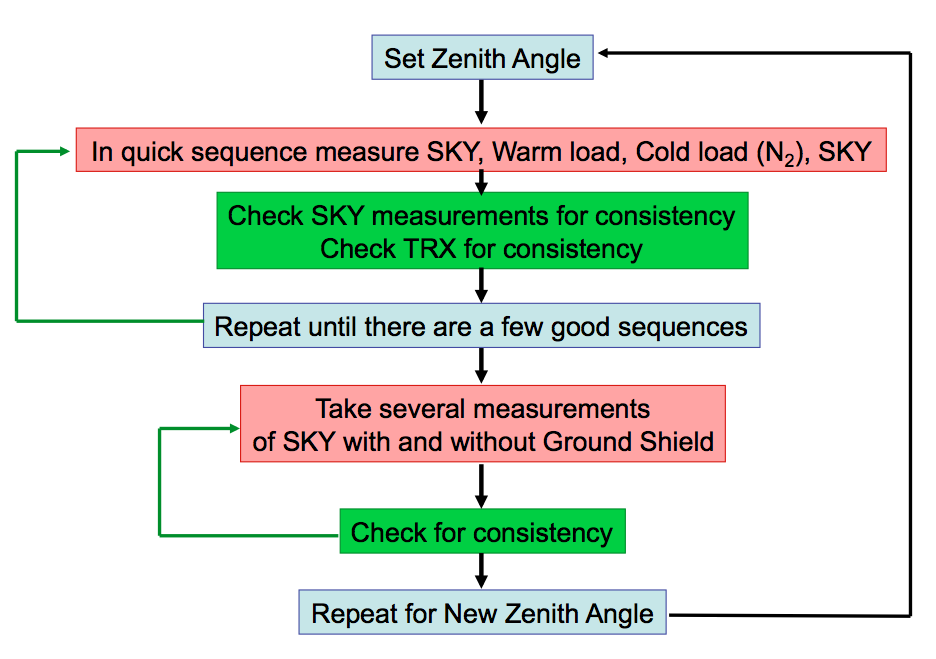
\includegraphics[trim=0pt 0pt 0pt 0pt,width=0.95\textwidth]{cmb/cmb-lab-flow-chart.png}
		\caption{Flow chart for taking sky data. It is important to make sure you obtain consistent results for each elevation angle. The ratio of the power on ambient to liquid nitrogen load should be very stable, since the scale factor $\alpha$ in Eq.~\ref{one} cancels in the ratio.  If the ratio is not stable there is a problem with the instrument (or liquid nitrogen load was not full immersed) and you will not get reliable results for Cosmic Microwave Background results.  The ratio of the output power for the ambient load to the nitrogen cooled load should be about 3.4 to 3.6, depending on the temperature of the ambient load. The typical receiver temperature should be around 11 K.  On a cloudy day the sky measurements may not be stable enough to achieve reliable results.  Why is that? \textit{Hint, light at cm wavelengths is also known as microwave radiation.  What is it that your microwave oven is heating up? And, if it absorbs the microwave radiation, then it must also emit it.}}
		\label{fig:flow-chart}
	\end{center}
\end{figure}

\section{Analysis}

\begin{steps}
	\item\label{cmb:step:plot} Plot your data, $T_\textrm{Sky}$ vs. airmass, with airmass on the horizontal axis. Airmass is defined as
	\begin{equation}
	 A(z) = \sec(z),
	\end{equation}
	where $z$ is the elevation angle.
	
	\item\label{cmb:step:fit} Fit your data to a line and record the slope and intercept for the line. \textit{Tip: double check your units. For elevation angle, we usually measure angles in degrees, but most calculators expect units of radians. Also, we will measure all temperatures in Kelvin.}
\end{steps}

\section{Report checklist and grading}

Each item below is worth 10 points, and there is an additional 10 points for attendance and participation.

\begin{itemize}
	\item Data and determination of temperature of two items inside the lab.
	
	\item Data table from Step~\ref{cmb:step:table}.
	
	\item The plot and fit parameters from Steps~\ref{cmb:step:plot} and \ref{cmb:step:fit}.
	
	\item Does your data agree with the model where the emission is dominated by the atmosphere?  What value to get for any residual temperature ($T_\textrm{CMB}$) and how do you interpret it?
	
	\item What are some of the uncertainties associated with your measurement? What steps did you take to measure or mitigate these uncertainties?
	
	\item Write a paragraph discussing the quality of your data and the historical significance of the Penzias and Wilson measurement. Include a discussion of the following: What was the context of the Penzias and Wilson measurement? Why was this measurement important? What were some of the competing cosmological theories at that time and how did the Penzias and Wilson measurement fit in to that context?
\end{itemize}